% Dokumtent start
\documentclass[%
  a4paper,%
  12pt,% <10pt, 9pt>
  %style=screen,
  %sender=bottom,
  blue,% <orange, green, violet>
  %rgb, <cmyk>
  %mono,
  %extramargin,
  %marginleft, <marginright>
  ]{tubsartcl}
\usepackage[utf8x]{inputenc}

\usepackage[ngerman]{babel}

\usepackage{lipsum}

% Titelseiten-Elemente
\title{Beispieltitel}
\subtitle{Untertitel}
\author{Max Mustermann\\\large{Straße}}
%\logo{Institut fuer Lorem Ipsum}
\logo{
\includegraphics{img/dummy_institut.pdf}}
\titleabstract{\lipsum[2]}
\titlepicture{infozentrum.jpg}


\begin{document}

\maketitle%[<plain/image/imagetext>,<logo=left/right>]

\tableofcontents
\newpage

\section{Uzftzfft purus elit}
\subsection{Meiune unterünerdchit}
Hier ist einfac ein Beispieltext mit gewissen Zeichen.\\
Hiwer schreibe ich weiter\\
\textbf{Hier} schreiben wir weiter...

\textcolor{tubsViolet}{Hier weiter mit Farbe ...}

\textcolor{tubsSecondaryLight80}{Dies ist ein Text in \texttt{tubsSecondary}.}
\textcolor{tubsViolet}{Dies ist ein Text in \texttt{tubsViolet}.}
\textcolor{tubsGreenDark}{Dies ist ein Text in \texttt{tubsGreenDark}.}\bigskip

%\lipsum[1]

\begin{figure}
\centering
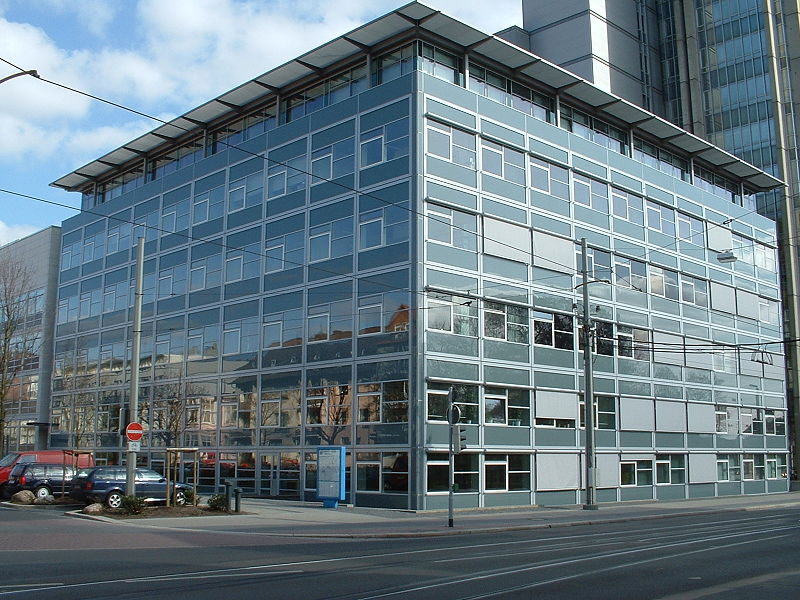
\includegraphics[width=0.7\linewidth]{infozentrum}
\caption{Das ist meine 1. Bild}
\label{fig:infozentrum}
\end{figure}

\begin{itemize}
	\item Punkt
	\item Punkt 2
\end{itemize}

$ x_{1}  = \frac{\sum x + 1}{y^{4}} $

\begin{itemize}
  \item Aufzählungspunkt Eins
  \item Aufzählungspunkt Zwei
    \begin{itemize}
      \item Unter-Aufzählungspunkt Eins
      \item Unter-Aufzählungspunkt Zwei
    \end{itemize}
  \item Aufzählungspunkt Drei
\end{itemize}

\section{Phasellus eu tellus sit amet}
\subsection{treerde}
\lipsum[2-5]

\section{Nulla malesuada porttitor diam.}

\lipsum[1-3]

\subsection{Donec felis erat}

\lipsum[4-7]

\end{document}
